\documentclass[14pt]{article}
\usepackage[utf8]{inputenc}
\usepackage{amsmath} % for using & and align formulas
\usepackage{parskip} % new paragraph adds a blank line before
\setlength{\parindent}{0in} % no indent
\renewcommand{\familydefault}{\sfdefault} %change font to ss
\usepackage{graphicx} %include images

\begin{document}
\section{High Level View}

On its core, Machine Learning about is a program that changes from exposure to data (experience).

Normally, data and parameters are the input to the model (mathematical function). This outputs a prediction, that we use to update the parameters in such a way that it better fits the data.

Deep Learning models complex patterns of data. It's particularly useful for non-linear patterns. This opens up a new space of problems to solve. Because Deep Learning is a part of Machine Learning, the previous logic is found neural network diagrams.

Network Diagrams can be found in section \ref{section:figs} 

\section{The steps}
There are two main steps: \textit{forward} and \textit{backward} propagation. 

Suppose a mathematical function is given to us:
$$ \hat{y}(x_1,x_2) = a x_1 + b x_2 + c$$
where $a$, $b$, $c$ are \textit{parameters}.

In \textbf{Forward Propagation} we initialize a set of parameters (say $a,b,c=0$), and use the equation to estimate the real output ($y$). Both values are input to ``$C(y, \hat{y})$'' which is small if we're doing well, or large if bad. 

So forward propagation is the calculation of $\hat{y}$ and $C(y,\hat{y})$ whatever shape they happen to have. 

In the next chapters $y$, $\hat{y}$ are $a$ and $\hat{a}$; this is just the notation used in ML/DL.

In \textbf{Backward Propagation} we minimize $C$, by differentiation, and find a way to move our function parameters towards the minimum of $C$. We use \textit{Gradient Descent} for this task.

The simplest neural network is the single layer. Later, hidden layers are included, from 1 (shallow network), to many (deep network).

We will see examples in detail, starting with multivariable linear regression, that is, a previous step to \textit{Deep Learning}.

\section{Summary}
Calculate $\hat{y}$ which is an estimation of $y$, compute $C(y,\hat{y})$, and use this to update $\hat{y}$ parameters, iteratively.

\section{Figures}\label{section:figs}
\begin{figure}[h]
 \centering
 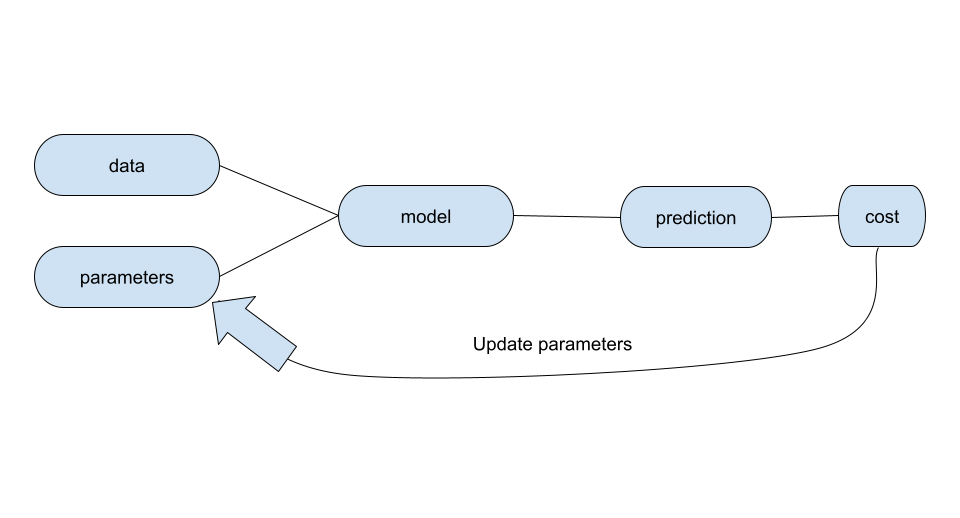
\includegraphics[width=0.9\textwidth]{ml.png}
  \caption{Machine Learning Process}\label{fig:learn}
\end{figure}

\begin{figure}
 \centering
 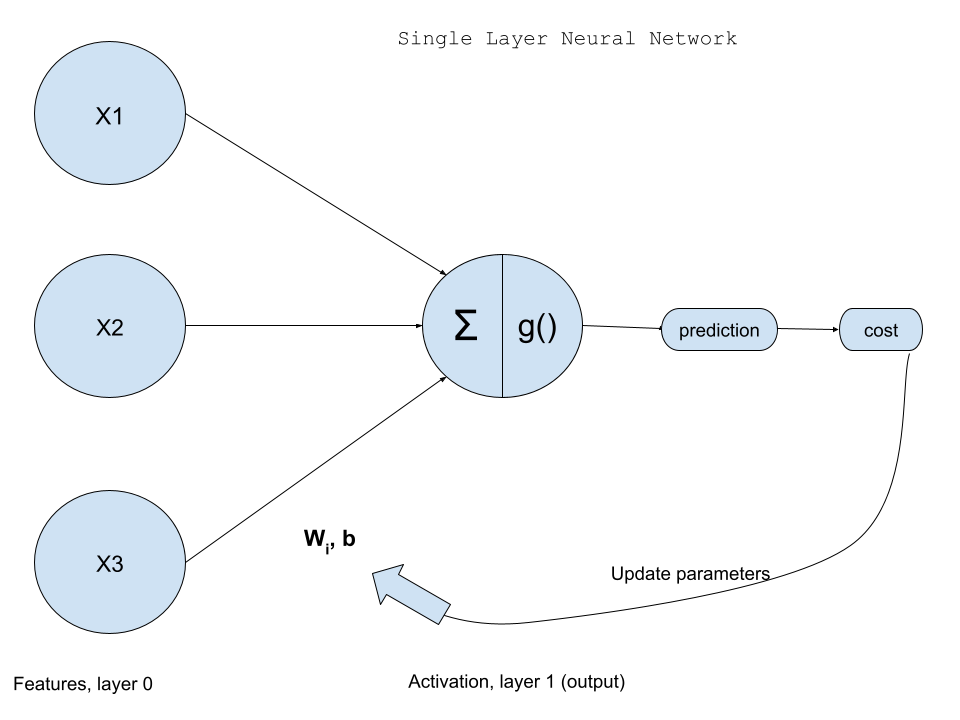
\includegraphics[width=\textwidth]{1L-NN.png}
 \caption{Single Layer Neural Network}
 \label{fig:single}
\end{figure}

\begin{figure}
 \centering
 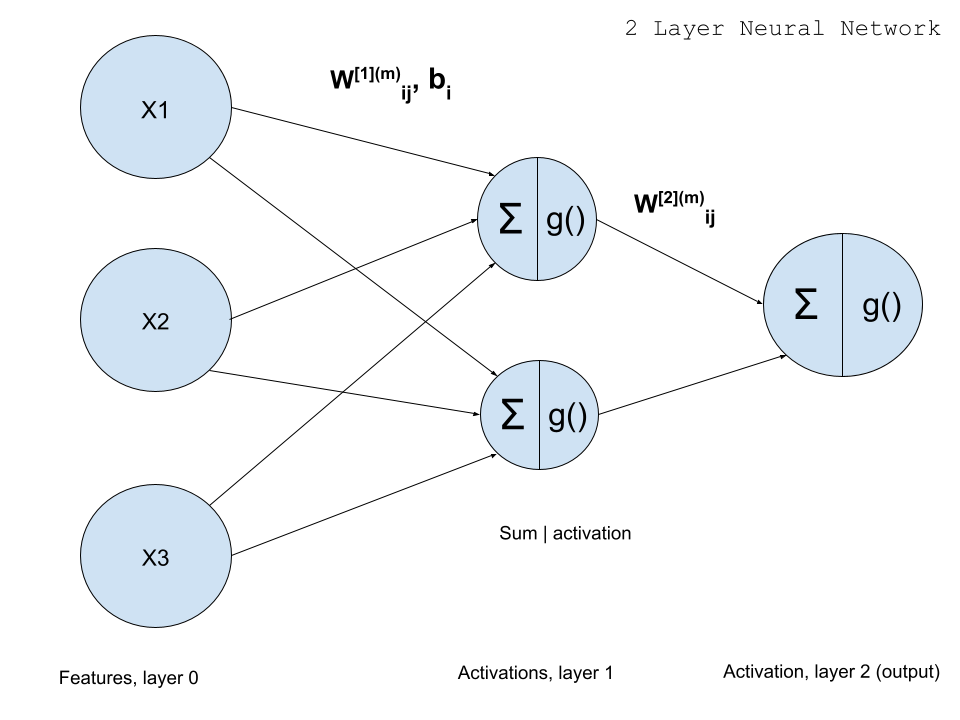
\includegraphics[width=\textwidth]{2L-NN.png}
 \caption{Shallow Neural Network}
 \label{fig:shallow}
\end{figure}

\section{Example: Multivariable Linear Regression}

A linear regression model for 2 features:
\begin{align*}
 y &= w_1\cdot x_1 + w_2\cdot x_2 + b \\
   &= \vec{w}\cdot\vec{x} + b
\end{align*}
$w_1$,$w_2$ control the slopes of this plane, $b$ translates it up and down. $\vec{x}$ is for one sample. Many samples are represented as a matrix:
\begin{align}
[y1, y2] = 
  [w1, w2]\cdot{}
  \begin{bmatrix}
  x_1 & x_1\\
  x_2 & x_2 
  \end{bmatrix}
 +  b
\end{align}
$y_i$ is the result for each sample (columns in the matrix).

We need to do forward and backward propagation.
\subsection{Forward Propagation}
The Loss $= Loss(w,b)$ in linear regression is the \textit{Square Error}:
\begin{align*}
  L_i(\vec{w}, b) &= (y_i - \hat{y})^2\\
  &=(y_i -\vec{w}\cdot{}\vec{x}_j -b)^2
\end{align*}

In Linear Regression, the cost is the averaged sum of $L_i$, and it's the \textit{Mean Square Error}:
\begin{align}
  C(w_1, w_2, b) &= \frac{1}{2} \sum_{i=0}^{i=2} L_i(w_1, w_2, b)\\
  &= \frac{1}{2}([y_1, y_2] - [\hat{y}_1, \hat{y}_2])\cdot{}([y_1, y_2]-[\hat{y}_1, \hat{y}_2])\\
  &=\frac{1}{2}([y_1, y_2] - [w_1, w_2]\mathbf{X}-b)\cdot{}([y_1, y_2] - [w_1,w_2]\mathbf{X} -b) \label{cost}
\end{align}
$\frac{1}{2}$ is to average over examples. Equation \ref{cost} is what we implement into code.
Outliers may be critical on the effect of weights and biases.

In Python it'd look like:
\begin{center}
  \begin{verbatim}
  Y' = np.dot(w,X) - b
  cost = 1/2*np.pow(2,(Y-Y'))
  \end{verbatim}
\end{center}





\subsection{Backward Propagation}
We need the Cost's derivative to find better weights and bias. The complicated thing is keeping track of each step.
\begin{align}
  dC(\vec{w},b) &= \frac{dC}{d\vec{w}} + \frac{dC}{db}\nonumber\\
  &= d(\sum_{i=0}^{i=2}L_i) = \sum_{i=0}^{i=2}dL_i(\vec{w},b) \label{diffp}\\
  &=\sum_{i=0}^{i=2} \frac{dL_i}{d\vec{w}} + \frac{dL}{db}\nonumber
\end{align}
Equation \ref{diffp} makes use of linearity property of diff. We sum over columns (each sample). Now, pick up a column/sample $k$:
\begin{align*}
  L_k(\vec{w},b) &= (y_k - \hat{y_k})^2\\
    L_k &= A_k(w_1, w_2, b)^2\\
    dL_k &= 2\cdot{}A_k(w1,w2,b)\cdot{}dA_k
\end{align*}
We named $A_k$ to the difference $y_i-\hat{y}_i$.
So $dC$ was reduced to:
\begin{align}
  dC &= \frac{1}{2}\sum_{i=0}^{i=2} dL_i\\
  &= \frac{1}{2}\times{}2\cdot{}A_i(w_1, w_2, b)\cdot{}dA_i
\end{align}
Where $A_i$ will be broadcasted, the shape is $1\times{}m$ and the sape of $dA_i$ is $n\times{}m$. Right now, $m=2$. The next step will be to sum over colums. And although $A_i$ will be calculated ($y_i - \hat{y}_i$) in the code, we need it now to find $dA_k$:
\begin{align*}
  dL_k  &= 2A_k\cdot{}(\frac{dA_k}{dw_1} + \frac{dA_k}{dw_2} + \frac{dA}{db}) \\
  A_k &= A_k(w_1, w_2, b)\\
  &= y_k - \vec{w}\cdot{}\vec{x_k} - b\\
  &= y_k - w_1\cdot{}x_{1k} - w_2\cdot{}x_{2k}-b\\
  dA_k &= -x_{1k} - x_{2k} -1
\end{align*}
where 
\begin{align*}
 \frac{dA_{k}}{dw_1} &= -x_{1k}\\ 
  \frac{dA_{k}}{dw_2} &= -x_{2k}\\ 
  \frac{dA_k}{db} &= -1
\end{align*} 

This can be expressed in compact form:
\begin{align}
  dC = \frac{1}{2}\times{}sum(2A\times(-\mathbf{X} -1))
\end{align}
Where ``sum'' implies we sum all values from the resulting array, and $b$ will be broadcast to the shape of $\mathbf{X}$.

We also found each partial derivative:
\begin{align}
  dC &= \frac{dC}{dw} = sum(dw+db)\\
 dC &= sum(2A\times{}\mathbf{X}) - sum(2A\times{}1)\\
\end{align}
To update the parameters, \textit{Gradient Descent} method is used. We update the vector $\vec{w}$ as follows:
\begin{align}
  \vec{w} &= \vec{w} -\frac{dC}{dw}\times{}d\vec{w}\cdot{}\alpha\\
  \vec{b} &= \vec{b} -\frac{dC}{db}\times{}d\vec{b}\cdot{}\alpha
\end{align}
$\alpha$ is called \textit{learning rate} and we use to tune the derivation. We go against the gradient so the sign is changed to $-$ (it points to max incresing direction otherwise).

\subsection{General Derivation}
The problem is to find $w_i, b$ such that the multidimensional "plane" has small error respect to each datapoint. Then for a new datapoint we will have a trained predictor.

In linear regression, the model is:
\begin{align*}
 y &= w_1\cdot x_1 + w_2\cdot x_2 +\ldots+ w_n\cdot x_n\\
   &= \sum_i^n w_i\cdot x_i + b \\
   &= \vec{w}\cdot\vec{x} + b
\end{align*}
Here $\vec{x}$ is for one sample. For $n$ samples, it becomes a matrix, we write $\vec{y} = \vec{w}\cdot\mathbf{X} + \vec{b}$. This is represented:
\begin{equation}
  [y_1 y_2 \ldots y_n] = 
  [w_1 w_2 \ldots w_n] \cdot
  \begin{bmatrix}
    x_{11} & x_{12} & \ldots & x_{1m}\\
    x_{21} & x_{22} & \ldots & x_{2m}\\
    \vdots & \vdots & \ddots & \vdots\\
    x_{n1} & x_{22} & \ldots & x_{nm}\\
  \end{bmatrix}
  + [b_1 b_2 \ldots b_n]
\end{equation}
There are $m$ examples-columns with $n$ features-rows. Hence $[\mathbf{X}] = m\times{}n$

The Loss $= L(w,b)$ in linear regression is the \textit{Square Error}:
\begin{align*}
  L(\vec{w},b) &= (y - \hat{y})^2\\
  &= (y_k - \vec{w}_j\cdot \vec{x}_j - b)^2
\end{align*}
The cost in any method/model measures how well it's doing with he current parameters. In Linear Regression, it is the averaged sum of $L_k$, and it's the \textit{Mean Square Error}:
\begin{align}
  C(\vec{w}, \vec{b}) &= \frac{1}{m}\sum_{i=0}^m L_i(\vec{w}, b)\\
  &=\frac{1}{m}\sum_{i=0}^m (\vec{y}_i - \vec{\hat{y}}_i)\cdot{}(\vec{y}_i - \vec{\hat{y}}_i)\\
  &= \frac{1}{m} (\vec{y} - \vec{w}\mathbf{X} - \vec{b})\cdot{}(\vec{y} - \vec{w}\mathbf{X} - \vec{b})
\end{align}
$C(\vec{w})$ is a way to denote $C$ depends on all the variables in $\vec{w}$. \textit{m} is the number of samples.

The cost is a ``bowl'', we will reach the global minimum (or close).
We use the Cost derivative to find the better weight and bias. 

\begin{align*}
  dC(\vec{w}, \vec{b}) &= \frac{dC}{dw} + \frac{dC}{db}\\
  &= \frac{1}{m} d(\sum^m_0 L_i)\\
  &= \frac{1}{m} \sum^m_{i=0} dL_i(\vec{w}, b_i)\\
  &= \frac{1}{m} \sum^m_{i=0} \frac{dL_i}{d\vec{w}} + \frac{dL_i}{db}\\
  &= \frac{1}{m} \sum^m_{i=0} \frac{dL_i}{dw_1} +\ldots +\frac{dL_i}{dw_n} + \frac{dL}{db}
\end{align*}

Take a particular column $k$:
\begin{align*}
  dL_k &= 2A * (\frac{dA}{dw_1}+ \frac{dA}{dw_2}+ \frac{dA}{db})\\
  A_k &= A(w_1, \ldots, w_n, b)\\
      &= y_k - \vec{w}\cdot{}\vec{x}_k - b \\
      &= y_k - w_1\cdot{}x_{1k}-\ldots{}-w_n\cdot{}x_{nk} - b \\
  dA_k &=  -x_{1k} -x_{2k} - x_{nk} -1 
\end{align*}
There is no graphical justification as to why we update $w$ and $b$ like that, but we are moving $w$ against (minus) the gradient multiplied by a constant (alpha) called \textit{learning rate}.

The minus sign is because the gradient always points away from the minimum and we want towards it (in one dimension there are only 2 directions). 

The process is called \textit{Gradient Descent}.

Because the $y_d - y_p$ is squared, MSE is a parabola for $b$ and $w$ then it makes sense: the farther away we are from the minimum the larger the gradient, and the more we want to update $w$ and $b$.






\section{Summary}

\begin{itemize}
 \item Model/Architecture*: equation to fit the data,
 \item FordP: Calculate the Cost, Evaluates the error,
 \item BackP: Training. Use cost, update $w$, $b$.
\end{itemize}
* Technically, model is only once the parameters are defined (after training). 
\begin{center}
Model =  Architecture + parameters (fixed ones). 
\end{center}

FP means from $X$ to $C$; BP from $L$ to $z$, in \textit{terms of the chain rule}.

\section{Other Concepts}
\textit{Overfitting}: Occurs when the cost in the training dataset decreases but it increases on the test dataset. The model starts to \textit{memorize} data, and does not \textit{generalize}.

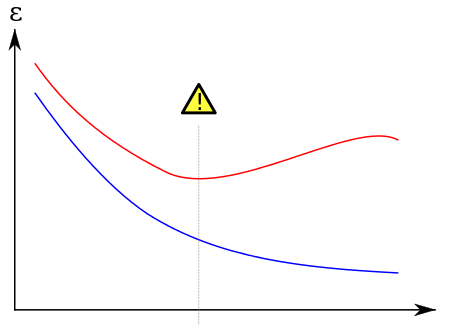
\includegraphics[width=\textwidth]{overfitting.png}

Training error: blue; validation error: red, both as a function of the number of training cycles. The best predictive and fitted model would be where the validation error has its global minimum.

\textit{Underfitting}: It occurs when the model or algorithm does not fit the data enough. It could be a bad model (too simple, or just not the right fit), or a lack of training, etc.

\textit{Classification v Regression}: A classification model is one which attempts to predict a class, or category. That is, it's predicting from a number of discrete possibilities, such as "dog" or "cat." A regression model is one which attempts to predict one or more numeric quantities, such as a temperature or a location. Which one we use depends on the nature of the variables.

\textit{Cross Validation}: The goal of cross-validation is to test the model's ability to predict new data that was not used in estimating it, in order to flag problems like overfitting or selection bias, and to give an insight on how the model will generalize to an independent dataset.

Why a CNN? It's the current state-of-the-art approach to creating computer vision models.

\section{High Level View}
Deep Learning is a Machine Learning area. The latter can be associated with the image, where update maps to learning in human terms, and more data maps to more experience (in human life). A program that learns from experience.

\begin{figure}
 \centering
 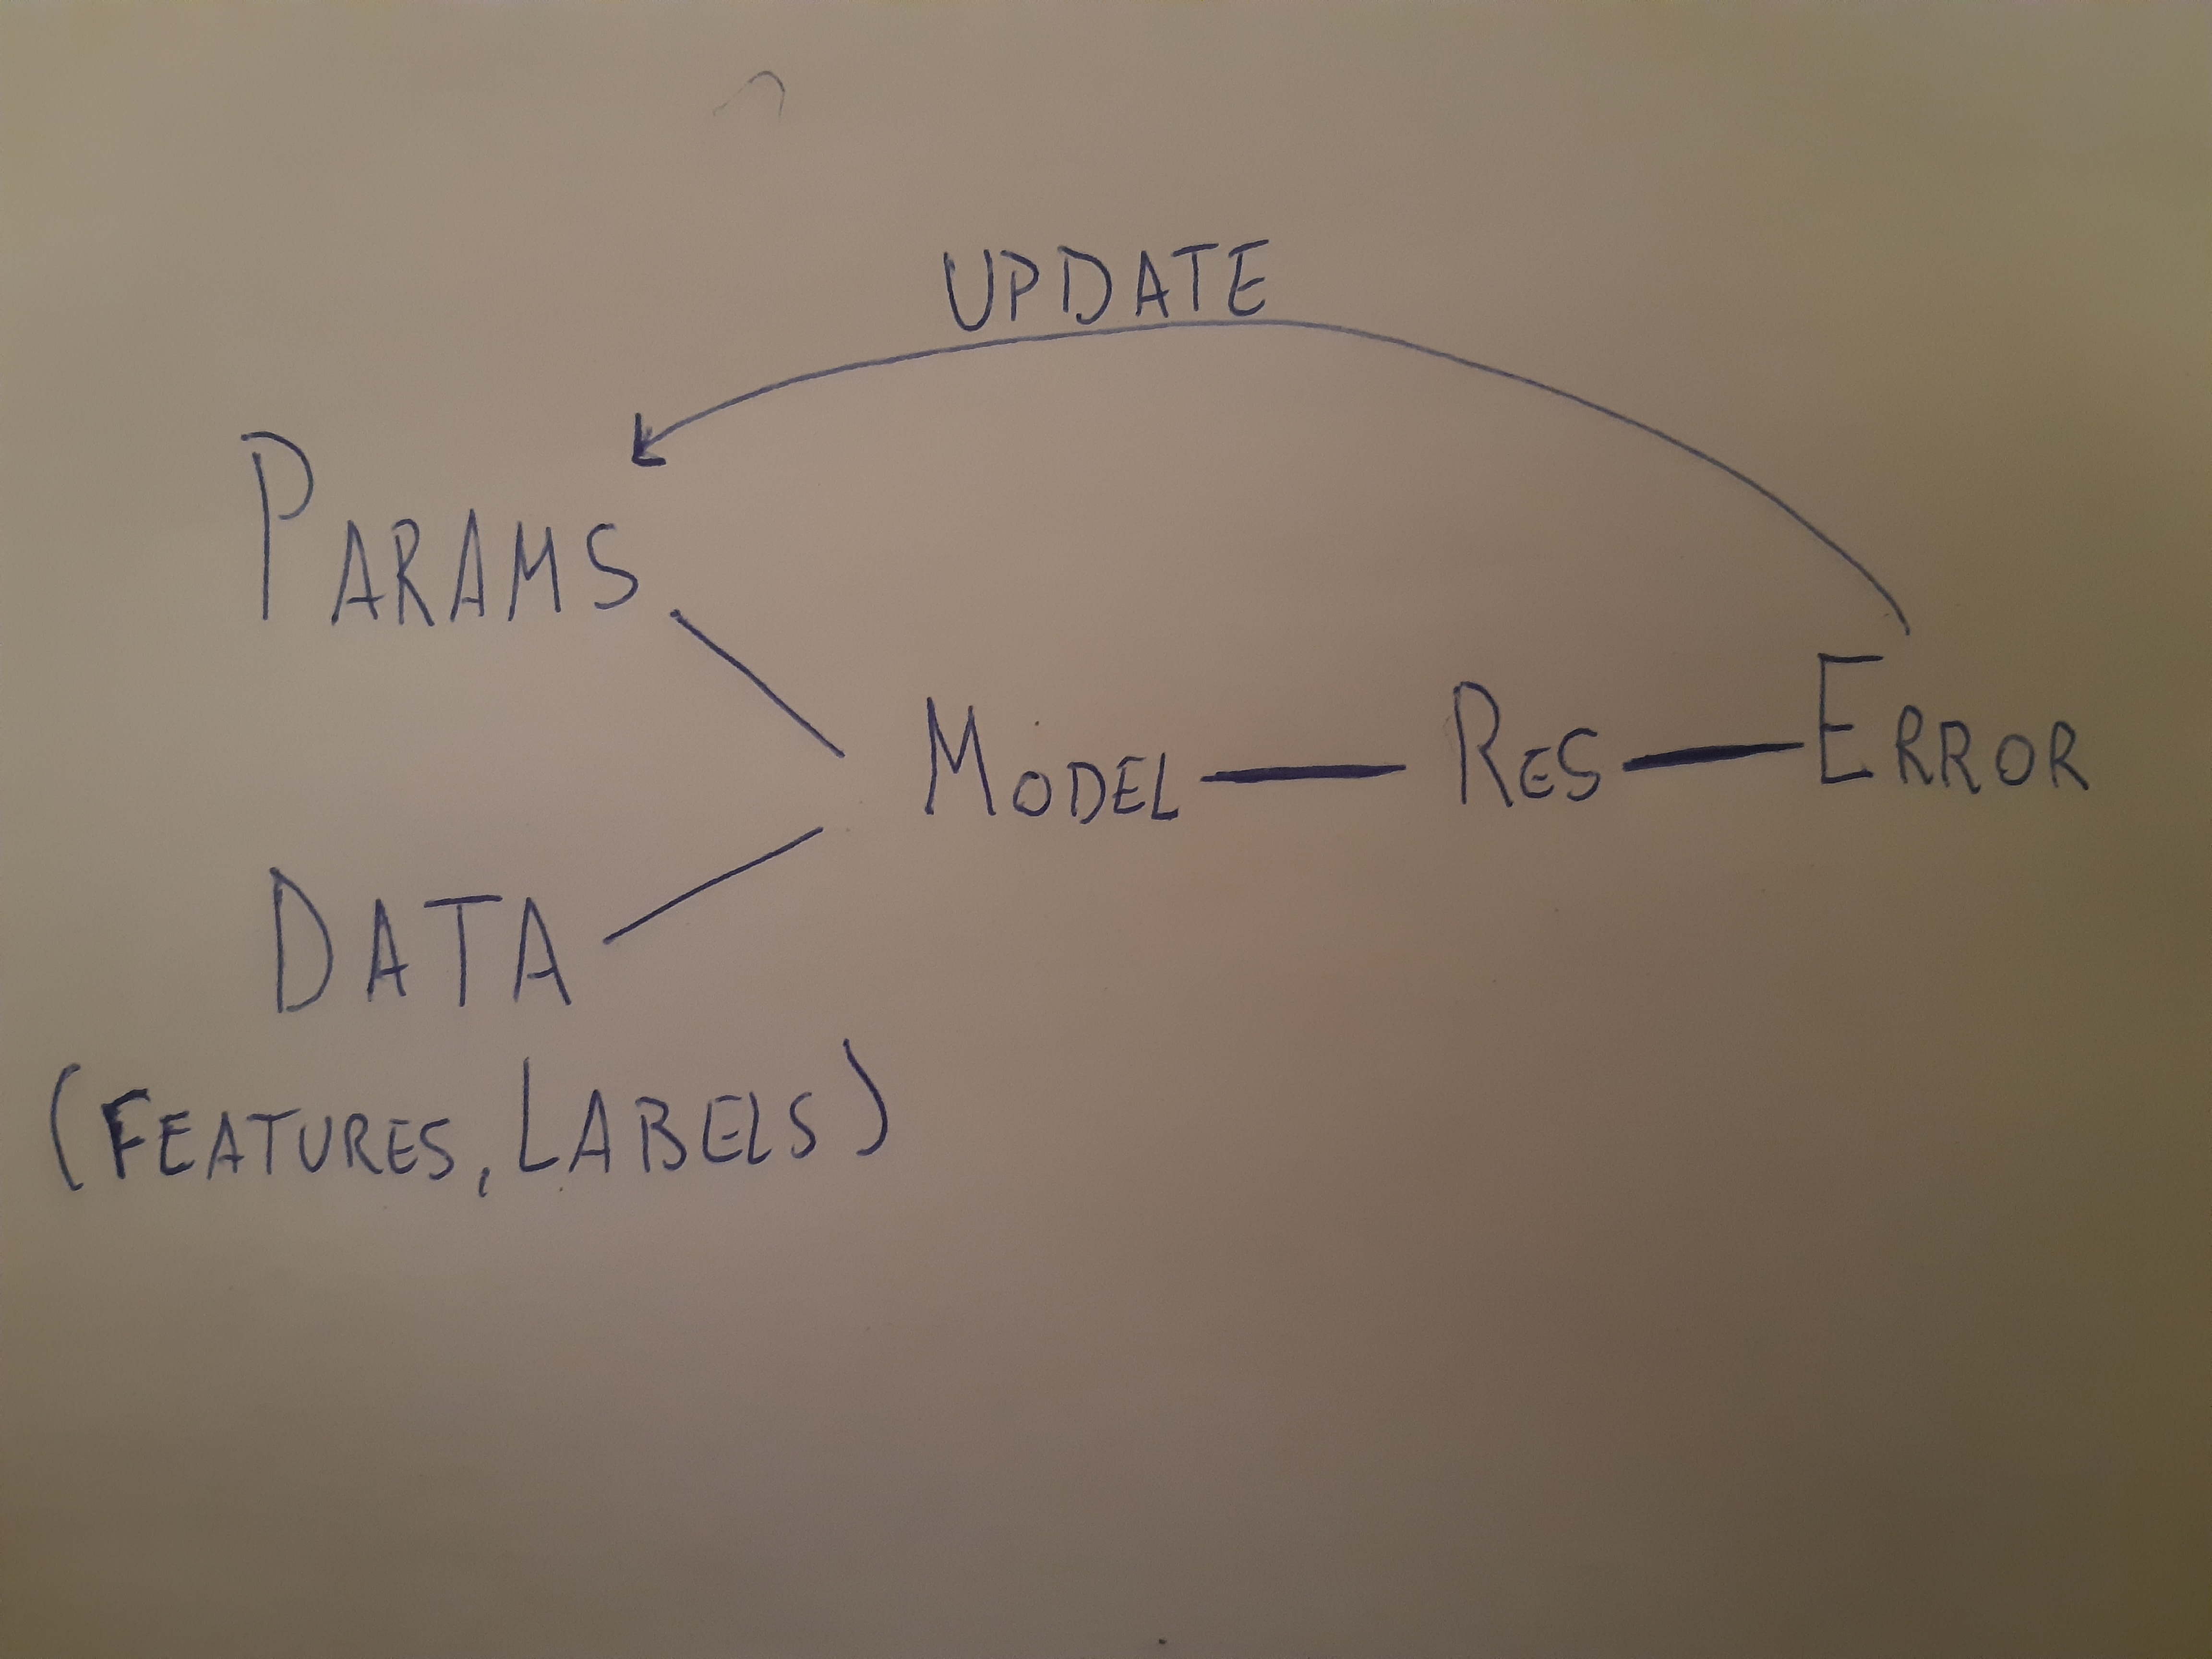
\includegraphics[width=0.9\textwidth]{ML.jpg}
 \caption{Machine Learning Process}
\end{figure}


\begin{figure}
 \centering
 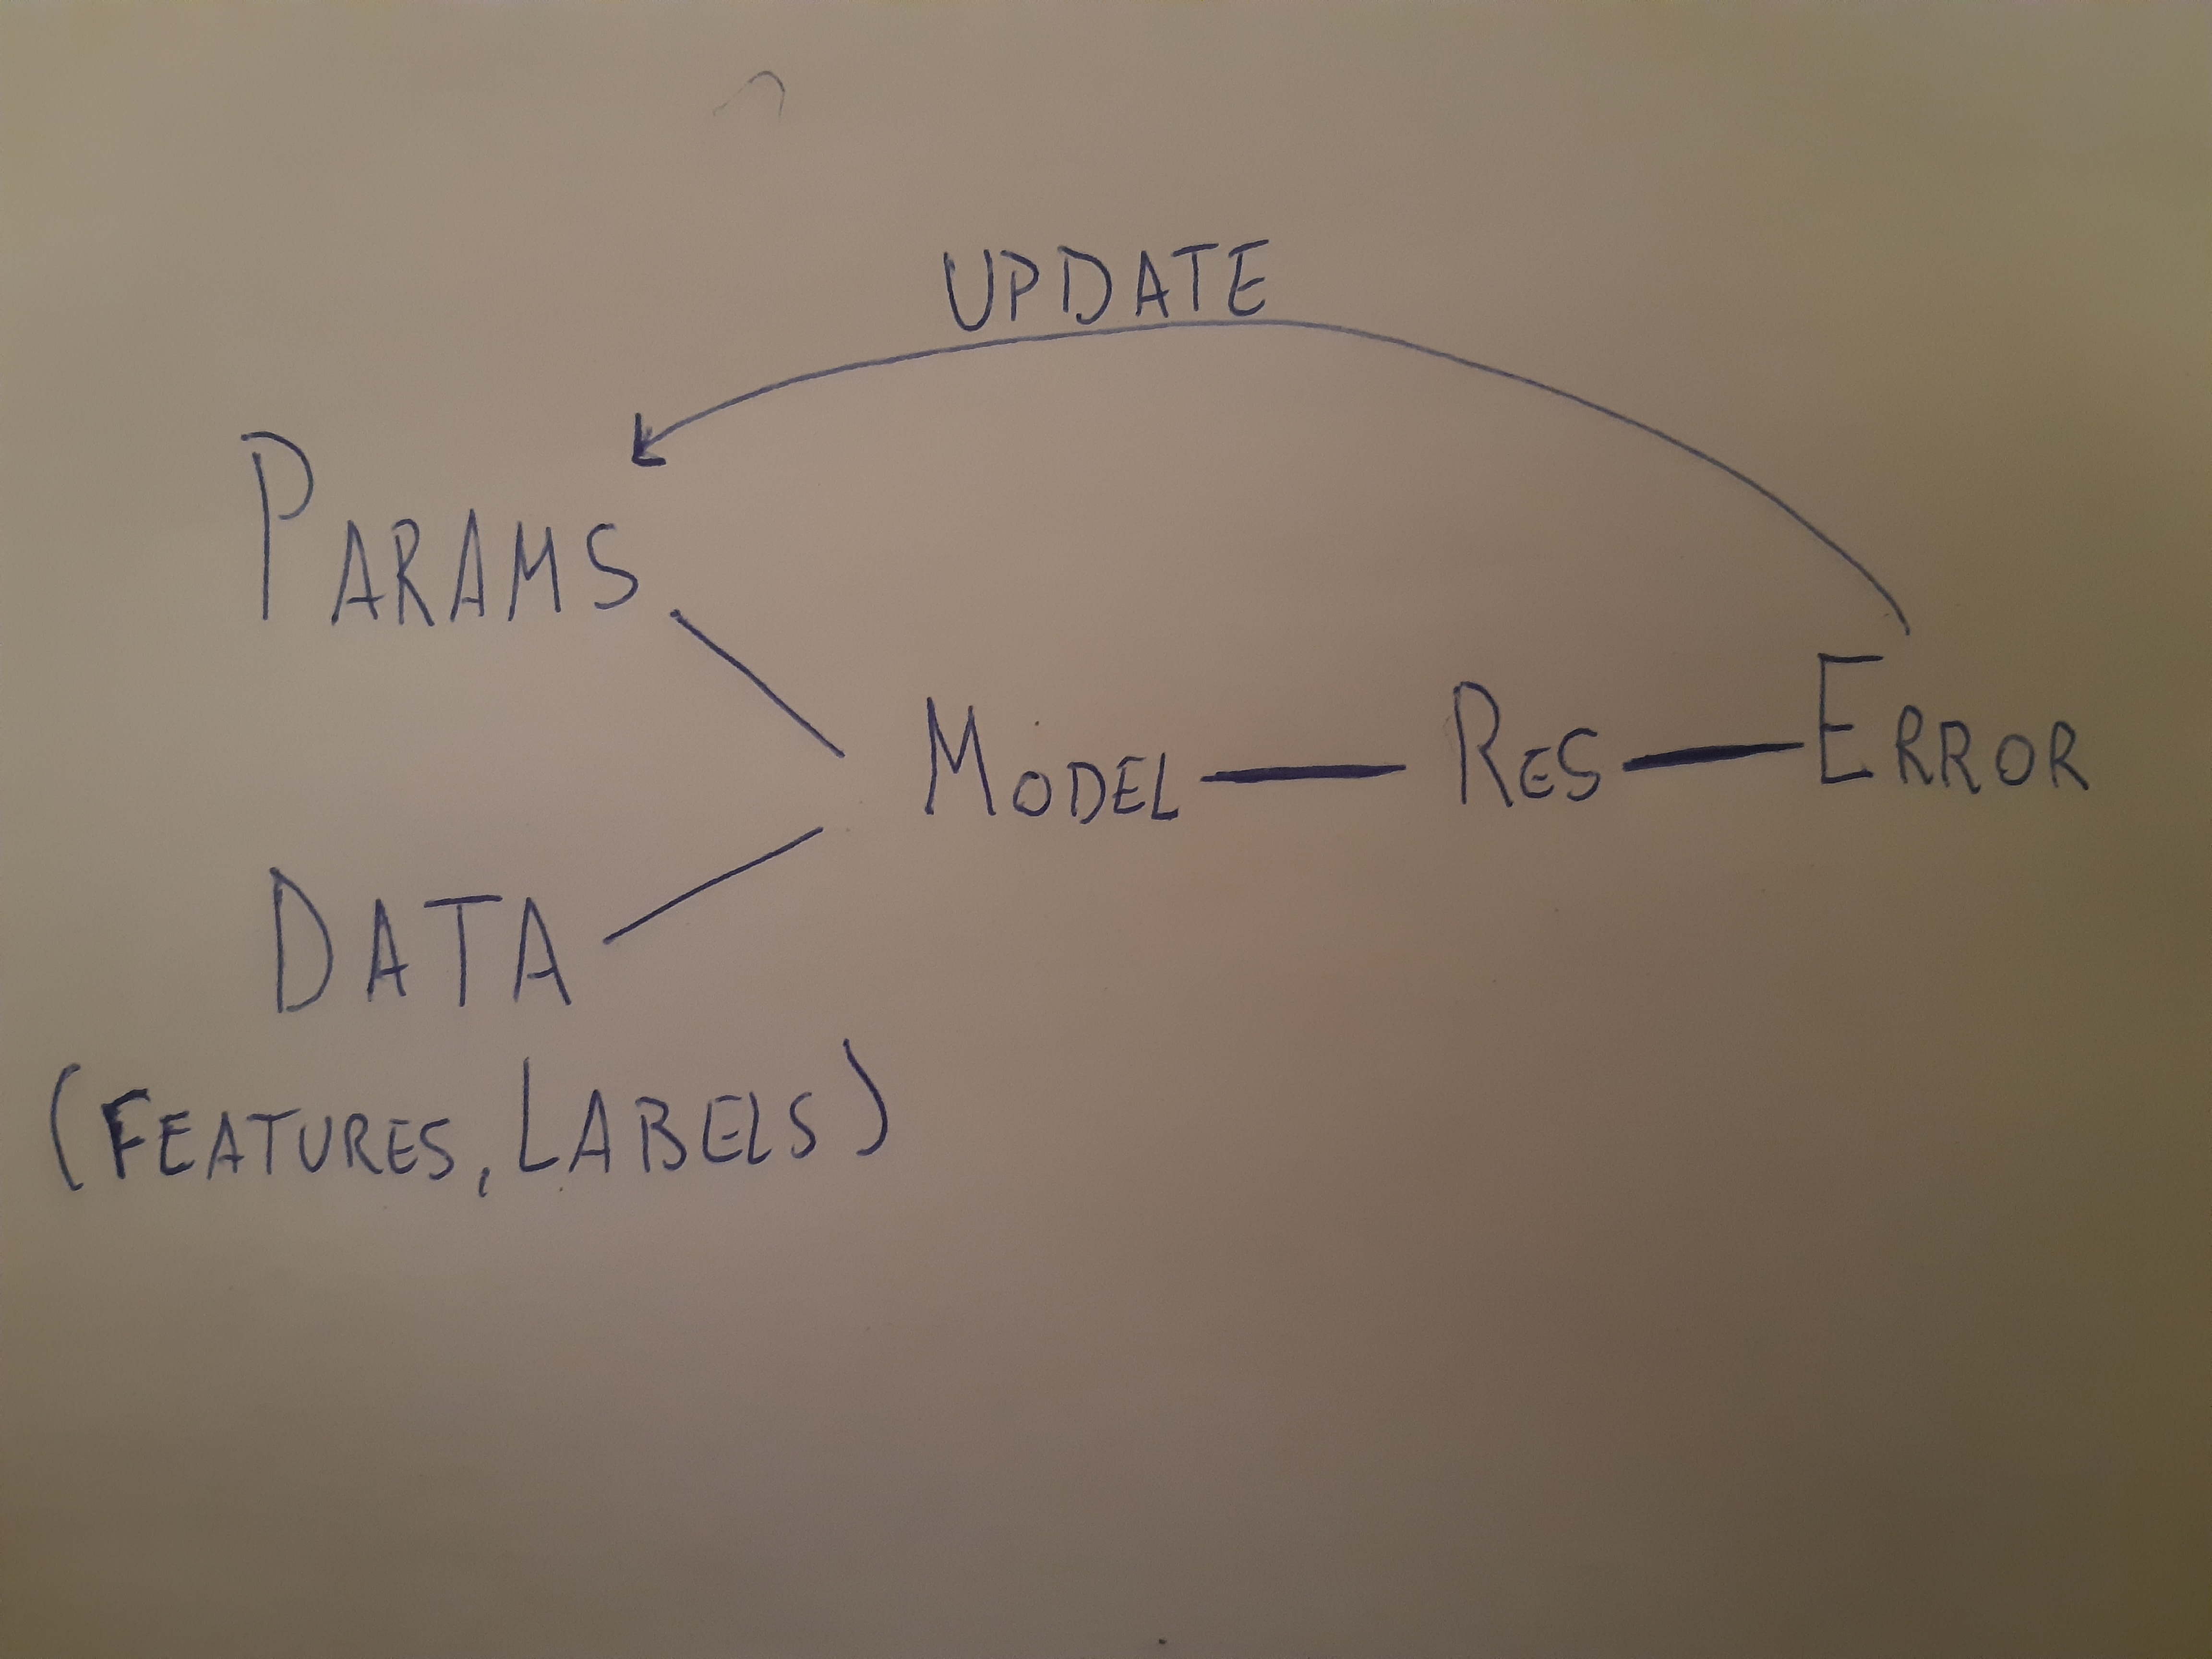
\includegraphics[width=0.9\textwidth]{ML.jpg}
 \caption{Two Layer NN}
\end{figure}


\end{document}
